\documentclass{article}

%%%%
% PLOTS mapas y conglomerados
% bibliografia
%%%%
\usepackage[utf8]{inputenc}
\usepackage{longtable}
\usepackage{authblk}
\usepackage{adjustbox}

\usepackage{natbib}



\title{LOS INDICES DEL MUNDO}
% autores
\renewcommand\Authand{, y }
\author[1]{\normalsize Santiago Serrano}
\author[2]{\normalsize Maria Luisa Franquis}

\affil[1,2]{\small  Escuela de Ingenier??a,Universidad de los Andes\\
\texttt{{delcurso,deallado}@uniandes.edu.col}}
\affil[1]{\small Instituto de altas investigaciones financieras\\
Banco del Parque\\
\texttt{delcurso@bp.com.col}}

\date{30 de Junio de 2018}

%%%%
\usepackage{Sweave}
\begin{document}
\input{paperVersion_6-concordance}

\maketitle


\begin{abstract}
Este es mi primer trabajo en exploracion y modelamiento de indices usando LATEX. Este trabajo lo he hecho bajo la filosof??a de trabajo replicable. Este es mi primer trabajo en exploracion y modelamiento de indices usando LATEX. Este trabajo lo he hecho bajo la filosof??a de trabajo replicable. Este es mi primer trabajo en exploracion y modelamiento de indices usando LATEX. Este trabajo lo he hecho bajo la filosof??a de trabajo replicable. Este es mi primer trabajo en exploracion y modelamiento de indices usando LATEX. Este trabajo lo he hecho bajo la filosof??a de trabajo replicable.
\end{abstract}

\section*{Introducci??n}

Aqui les presento mi investigacion sobre diversos indices sociales en el mundo. Los indices los consegu?? de wikipedia, espero que les gusten mucho. Aqui les presento mi investigacion sobre diversos indices sociales en el mundo. Los indices los consegu?? de wikipedia, espero que les gusten mucho.Aqui les presento mi investigacion sobre diversos indices sociales en el mundo. Los indices los consegu?? de wikipedia, espero que les gusten mucho.Aqui les presento mi investigacion sobre diversos indices sociales en el mundo. Los indices los consegu?? de wikipedia, espero que les gusten mucho.
Aqui les presento mi investigacion sobre diversos indices sociales en el mundo. Los indices los consegu?? de wikipedia, espero que les gusten mucho.Aqui les presento mi investigacion sobre diversos indices sociales en el mundo. Los indices los consegu?? de wikipedia, espero que les gusten mucho.Aqui les presento mi investigacion sobre diversos indices sociales en el mundo. Los indices los consegu?? de wikipedia, espero que les gusten mucho.

Comencemos viendo que hay en la secci??n \ref{univariada} en la p??gina \pageref{univariada}.

\clearpage



\section{Exploraci??n Univariada}\label{univariada}

En esta secci??n exploro cada ??ndice. En esta secci??n exploro cada ??ndice. En esta secci??n exploro cada ??ndice. En esta secci??n exploro cada ??ndice. En esta secci??n exploro cada ??ndice. En esta secci??n exploro cada ??ndice. En esta secci??n exploro cada ??ndice. En esta secci??n exploro cada ??ndice. En esta secci??n exploro cada ??ndice.





Para conocer el comportamiento de las variables se ha preparado la Tabla \ref{Tfrecuencias}, donde se describe la distribuci??n de las modalidades de cada variable. Los n??meros representan la situaci??n de algun pa??s en ese indicador, donde el mayor valor num??rico es la mejor situaci??n.

% latex table generated in R 3.5.0 by xtable 1.8-2 package
% Fri Jun 29 17:54:22 2018
\begingroup\normalsize
\begin{longtable}{llrrr}
\caption{Tablas de Frecuencia de la variables en estudio} \\ 
 \textbf{Variable} & \textbf{Levels} & $\mathbf{n}$ & $\mathbf{\%}$ & $\mathbf{\sum \%}$ \\ 
  \hline \hline
Departamento & Amazonas & 1 & 3.1 & 3.1 \\ 
   & Antioquia & 1 & 3.1 & 6.2 \\ 
   & Arauca & 1 & 3.1 & 9.4 \\ 
   & Atl

Como apreciamos en la Tabla \ref{Tfrecuencias}, los pa??ses en la mejor situaci??n son los menos, salvo en el caso del \emph{??ndice de libertas mundial}\footnote{N??tese que esto se puede deber a la {\bf menor} cantidad de categor??as.}

\clearpage

Para resaltar lo anterior, tenemos la Figura \ref{barplots} en la p??gina \pageref{barplots}. 


%%%%% figure
\begin{figure}[h]
\centering
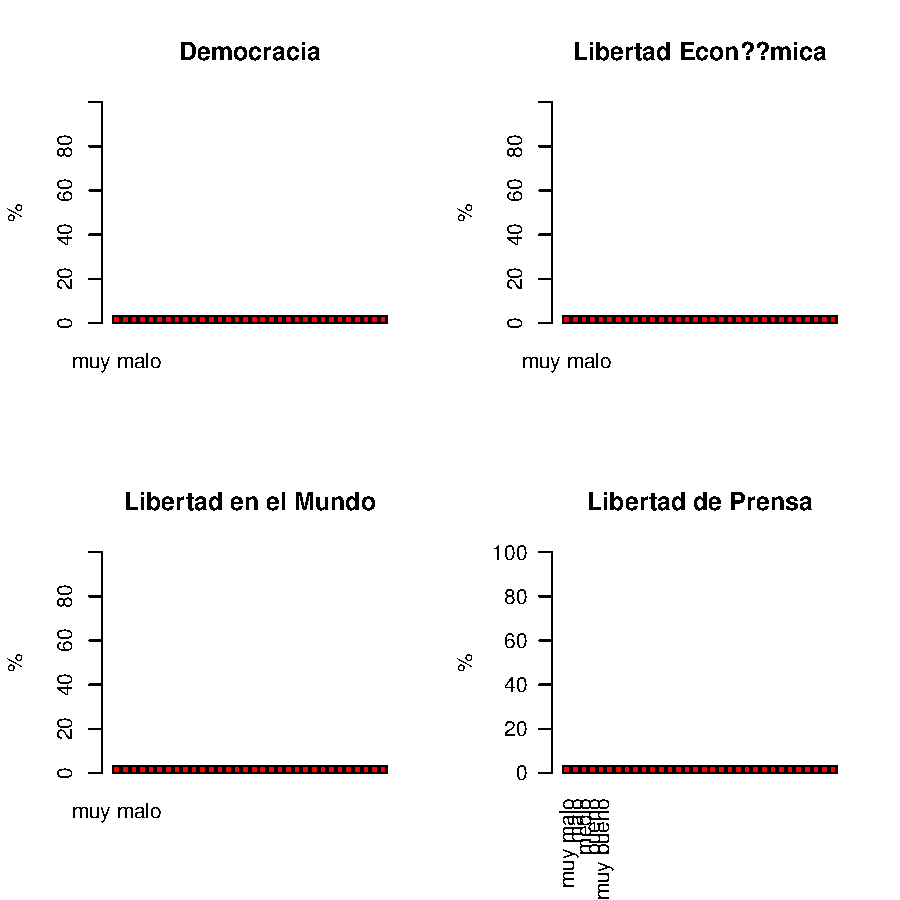
\includegraphics{paperVersion_6-barplots}
\caption{Distribuci??n de Indicadores}
\label{barplots}
\end{figure}

Adem??s de la distribuci??n de los variable, es importante saber el valor central. Como los valores son de naturaleza ordinal debemos pedir la {\bf mediana} y otras medidas de posici??n (como los \emph{cuartiles}, los que no pediremos pues son pocos valores). La mediana de cada variable la mostramos en la Tabla \ref{stats} en la p??gina \pageref{stats}.

% Table created by stargazer v.5.2.2 by Marek Hlavac, Harvard University. E-mail: hlavac at fas.harvard.edu
% Date and time: Fri, Jun 29, 2018 - 17:54:22
\begin{table}[!htbp] \centering 
  \caption{Medidas estad??sticas} 
  \label{stats} 
\begin{tabular}{@{\extracolsep{5pt}}lcc} 
\\[-1.8ex]\hline 
\hline \\[-1.8ex] 
Statistic & \multicolumn{1}{c}{N} & \multicolumn{1}{c}{Median} \\ 
\hline \\[-1.8ex] 
Poblaci..n.Cabecera & 32 & 717,197 \\ 
Poblaci..n.Resto & 32 & 268,111.5 \\ 
Poblaci..n.Total & 32 & 1,028,429 \\ 
\hline \\[-1.8ex] 
\end{tabular} 
\end{table} 

\section{Exploraci??n Bivariada}

En este trabajo estamos interesados en el impacto de los otros indices en el nivel de Democracia. Veamos las relaciones bivariadas que tiene esta variable con todas las dem??s:

